% !TeX root = ../main.tex
% Add the above to each chapter to make compiling the PDF easier in some editors.

\section{Reinforcement Learning}

The simplest examples of learning come from our own lives; we learn to walk, speak the language, or cook. All those activities span our entire life, it influences who we are and the decisions we take in life. We know that living animals such as mammals learn from their social and asocial interactions with the environment \cite{AnimalInt11}. 
Although we have not yet developed a full-scale theory of animal learning, we have developed computational objectives for machine learning \cite{Sutton2018}. 
This computational approach falls into three categories as supervised, unsupervised, and reinforcement learning. In this chapter, we will consider the Reinforcement Learning objectives and problem formulation.

Reinforcement learning provides a systematic approach to maximize the reward by linking observations to actions. A reinforcement learning agent creates its data by interacting with the environment. Therefore, it is fundamentally different from supervised and unsupervised learning, where the data is already provided \cite{Sutton2018}. 
Another critical difference is the inherent goal-oriented approach. The reinforcement learning agent maximizes the rewards to achieve its goal. Whereas, other machine learning approaches lack this goal \cite{Sutton2018}.
For instance, supervised learned software recognizing faces can be used for security reasons to detect criminals or can be easily used to unlock phones. However, a reinforcement learning agent trained to drive a car autonomously can only drive a car. In a sense, reinforcement learning provides us end-to-end learning.

A core feature of reinforcement learning is that it acts on uncertain environments and, in return, receives the observation and reward. Fundamentally, a learning agent collects this experience and tunes its action to increase the expected reward. The expected reward term refers to the end of the horizon. For example, a chess-playing agent can choose to sacrifice the queen in the next move for a checkmate in the move after. In this case, the reward would decrease when the agent loses a queen, but the agent's goal will be satisfied by terminating the game. For a well-defined reinforcement learning system, we can speak of four main components: Policy to decide the actions, a reward to maximize the expected reward in the horizon, and a model of the environment, describing which directions the chess pieces can move. The components of reinforcement learning are formulated based on Markov Decision Process. In the MDP chapter, we will detailly explain RL components. We will explain first Markov Chains, then MDP,  in the next chapters \cite{PerezMIT}.

\subsection{Markov Chain}

Markov chain has a strong correlation with the weak law of large numbers. This law has a tremendous significance on stochastic modeling. It states that the average of a large number of experimentations converges to the real value of the probability of a particular task. For example, if one tosses infinite amounts of the coin, the average number of heads should converge to 0.5 \cite{Gagniuc2017}. 
Bernoulli's weak law of large numbers only covers independent events. Markov proved that Bernoulli's law also holds on dependent cases \cite{Gagniuc2017}. 
As the law of large numbers suggests, if one conducts a large number of iterations on a problem, one can infer the transition matrix. This matrix proves to be the only information one needs to compute the next state.

This characteristic defines the famous Markov property; the current state captures all the necessary information to predict the next state. If we extrapolate this example to slightly complex systems, such as weather forecast, we need today's weather report to predict tomorrow's forecast, assuming that we know the transition matrix. Naturally, one can formulate other events with Markov Chain lawnmower, and a random walk is the straightforward examples in the literature\cite{Gagniuc2017}.

It is also possible to attach rewards to Markov Chain's formulation. In figure \ref{fig: markov_chain}, the transition between states is represented with the arcs. Moreover, each transition has a probability similar to the transition matrix; we defined before. Each state has an immediate reward and a value function. The immediate reward is received directly when the actor moves to that state. The value of a state represents how likely the future actor will end up collecting high rewards. 

\begin{figure}[htbp]
    \centering
    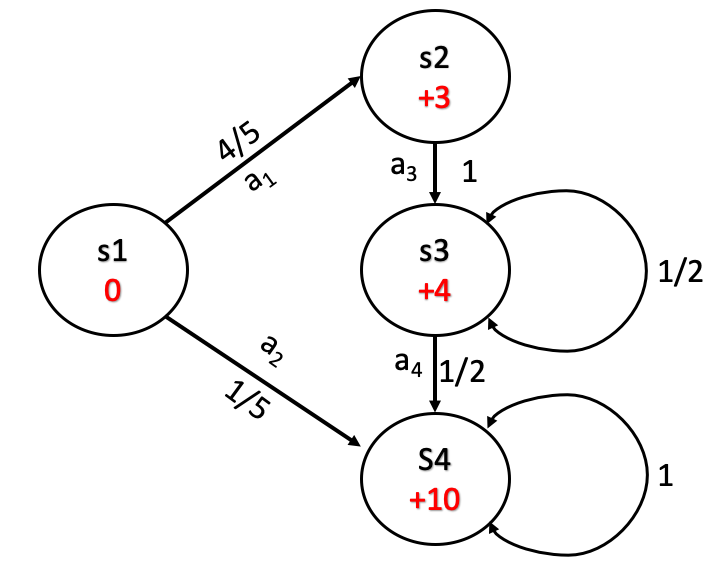
\includegraphics[width=0.5\textwidth]{figures/markovchain}
    \caption{Markov chain with transition probabilties and rewards}
    \label{fig: markov_chain}
\end{figure}

The value of a state will be later significant to solve Reinforcement Learning problems through Value Iteration methods. They are one of the essential algorithms that led to the initial success of reinforcement learning research.
